\documentclass[slide05.tex]{subfiles}
\begin{document}
\begin{frame}
    \centering
    \frametitle{VLC メディアプレイヤーを開こう}
    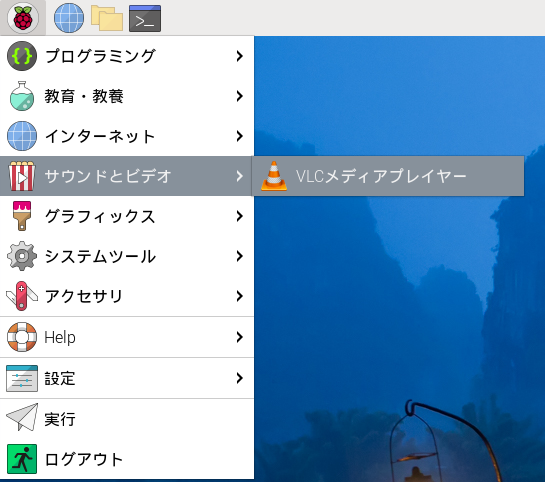
\includegraphics[height=0.7\textheight,keepaspectratio]{../../asset/image/launch_vlc.png}

    デスクトップでもスライドが見られるようにします。
\end{frame}

\begin{frame}
    \centering
    \frametitle{「メディア」→\\「ネットワークストリームを開く」}

    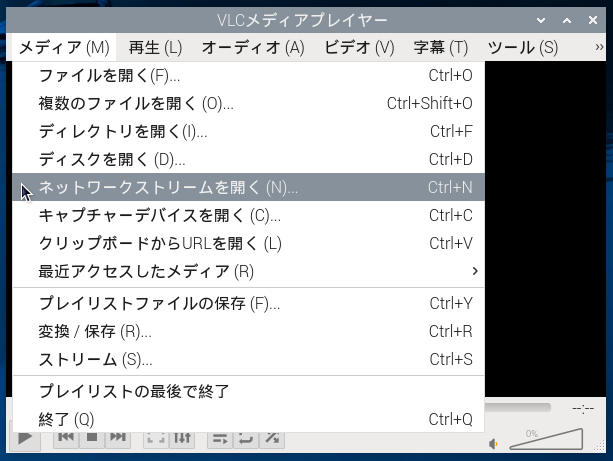
\includegraphics[height=0.7\textheight,keepaspectratio]{../../asset/image/open_network_stream.png}
\end{frame}

\begin{frame}[fragile]
    \centering
    \frametitle{配信 URI を入力して「再生」}

    \begin{lstlisting}[language={},basicstyle=\huge\ttfamily]
udp://@239.1.1.1:1234
    \end{lstlisting}

    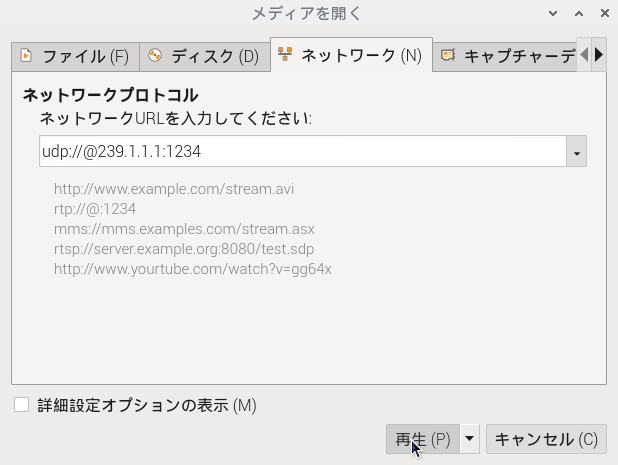
\includegraphics[height=0.6\textheight,keepaspectratio]{../../asset/image/set_streaming_uri.png}
\end{frame}
\end{document}
